% !Mode:: "TeX:UTF-8"

\begin{frame}
	\frametitle{第八讲、空间曲面与曲线习题课}
	\linespread{1.5}
	\begin{enumerate}
	  \item {\bf 内容与要求}%{\color{blue}( \S7.3-7.4 )}
	  \begin{itemize}
	    \item 空间曲面与曲线的一般式方程
	    \item 空间曲面与曲线的参数方程
	    \item 旋转曲面
	    \item 二次曲面及其标准方程
	    \item 空间曲线的投影
% 	    \item 熟练掌握常见的一阶常微分方程的解法
% 	    \begin{itemize}
% 	      \item 可分离变量方程
% 	      \item 齐次方程
% 	      \item 一阶线性方程
% 	    \end{itemize}
	  \vspace{1em}
	  \end{itemize}
% 	  \item {\bf  课后作业:}
% 	  \begin{itemize}
% 	    \item {\b 习题7.3:1(1,4,6),2(3,5),3,5}
% 	    \item {\b 习题7.4:3,4,5,6(1,5),8(1),9(1)}
% 	  \end{itemize}
	\end{enumerate}
\end{frame}

% \begin{frame}{补充例题}
% 	\linespread{1.5}
% 	\begin{exampleblock}{{\bf 例1}\hfill}
% 		求与直线$L_1:y=0,z=a$和$L_2:x=0,z=-a$均相切的球面中心的轨迹,并判断其形状。
% 	\end{exampleblock}\pause
% 	{\bf 注:}\alert{双曲抛物面是到两条垂直直线距离相等的点的轨迹}\pause
% 	\bigskip
% 	\begin{exampleblock}{{\bf 例2}\hfill}
% 		求与点$A(1,-1,1)$和点$B(-2,2,1)$距离之比为$1:2$的点的全体满足的方程。
% 	\end{exampleblock}
% \end{frame}

\begin{frame}
	\linespread{1.2}
	\begin{exampleblock}{{\bf 例1}\hfill}
		求球面$x^2+y^2+z^2=r^2$与以下曲面的交线的参数方程:
		\begin{enumerate}
		  \item $x^2+y^2=a^2$
		  \item $x^2+y^2=az^2$
		\end{enumerate}
	\end{exampleblock}
	\pause
	\bigskip
	\begin{exampleblock}{{\bf 例2}\hfill}
		求曲线$\left\{\begin{array}{l}
			x^2-y^2=2z+1\\
			x+y=z
		\end{array}\right.$
		的参数方程。
	\end{exampleblock}
\end{frame}

\begin{frame}
	\linespread{1.5}
	\begin{exampleblock}{{\bf 例3}\hfill P54-8}
		证明:到定直线及该直线上一定点的距离平方和为常数的动点轨迹为一个旋转曲面。
	\end{exampleblock}
	\pause
% 	{\bf 注:}\alert{双曲抛物面是到两条垂直直线距离相等的点的轨迹}\pause
	\bigskip
	\begin{exampleblock}{{\bf 例4}\hfill P55-9}
		已知点$A(1,0,0)$与点$B(0,1,1)$,直线$AB$绕$z$轴旋转一周所成的旋转曲面为
		$S$,求$S$与$z=0$、$z=1$所围成的立体体积。
	\end{exampleblock}
\end{frame}

\begin{frame}
	\linespread{1.2}
	\begin{exampleblock}{{\bf 例5}\hfill}
		求直线
		$$l:\df{x}{a}=\df{y-b}0=z$$绕$z$轴旋转一周所得曲面方程,并指出该曲面
		的类型。
	\end{exampleblock}
% 	\pause
% 	\bigskip
% 	\begin{exampleblock}{{\bf 例6}\hfill P55-例9}
% 		已知点$A(1,0,0)$与点$B(0,1,1)$,直线$AB$绕$z$轴旋转一周得到曲面$S$,求
% 		$S$及两平面$z=0,z=1$所围立体的体积。
% 	\end{exampleblock}
\end{frame}

\begin{frame}{问题分析}
	\linespread{1.2}
	\begin{exampleblock}{{\bf 例6}\hfill}
		求空间曲线$$\left\{\begin{array}{l}
		F(x,y,z)=0\\ G(x,y,z)=0
		\end{array}\right.$$绕直线
		$$\df{x-a}m=\df{y-b}n=\df{z-c}p$$
		旋转一周所得曲面的方程。
	\end{exampleblock}
\end{frame}

\begin{frame}
	\linespread{1.2}
	\begin{exampleblock}{{\bf 例7}\hfill P68-10}
		证明:空间曲线$\Gamma:x=\varphi(t),y=\phi(t),z=\psi(t)$绕$z$轴旋转一周所得
		旋转曲面的参数方程为:
		$$\left\{\begin{array}{l}
			x=\sqrt{\varphi^2(t)+\phi^2(t)}\cos\theta,\\
			y=\sqrt{\varphi^2(t)+\phi^2(t)}\sin\theta,\\
			z=\psi(t)
		\end{array}\right.$$
	\end{exampleblock}
\end{frame}

\begin{frame}
	\linespread{1.5}
	\begin{exampleblock}{{\bf 例8}\hfill}
		设柱面的母线平行于直线$x=y=z$,准线为$x+y-z=1,x-y+z=0$,求柱面的方程。
	\end{exampleblock}\pause
	\bigskip
	\begin{exampleblock}{{\bf 例9}\hfill}
		求通过曲线$\left\{\begin{array}{l}
			x^2+y^2+z^2=8\\
			x^2+z^2-y^2=0
		\end{array}\right.$,且母线分别平行于$x$轴,$y$轴和$x=y=z$的柱面方程。
	\end{exampleblock}
\end{frame}

\begin{frame}
	\linespread{1.2}
	\begin{exampleblock}{{\bf 例10}\hfill}
		求由不等式组
		$$x\geq 0,\;y\geq 0,\;z\geq 0,\;x+z\leq 1,\; y^2+z^2\leq 1$$
		所确定的立体体积。
	\end{exampleblock}
\end{frame}

\begin{frame}
	\linespread{1.5}
	\begin{exampleblock}{{\bf 例11}\hfill}
		由椭球面$\df{x^2}{a^2}+\df{y^2}{b^2}+\df{z^2}{c^2}=1$的中心引三条相互垂直的射线,
		分别交椭球面于三点$P_i(i=1,2,3)$,记$|\bm{OP}_i|=r_i(i=1,2,3)$,证明:
		$$\df{1}{r_1^2}+\df{1}{r_2^2}+\df{1}{r_3^2}
		=\df{1}{a^2}+\df{1}{b^2}+\df{1}{c^2}$$
	\end{exampleblock}
\end{frame}

\begin{frame}
	\linespread{1.2}
	\begin{exampleblock}{{\bf 例12}\hfill}
		求直线
		$$L:\left\{\begin{array}{l}
			x+y+z-1=0\\
			x-y+z+1=0
		\end{array}\right.$$
		在平面$\pi:x+2y-z=0$上的投影直线方程,并求该直线绕$z$轴旋转一周所得
		旋转曲面的方程。
	\end{exampleblock}
\end{frame}

\begin{frame}
	\linespread{1.2}
	\begin{exampleblock}{{\bf 例13}\hfill}
		试确定$\lambda$为何值时,平面$x+\lambda z-1=0$与单叶双曲面
		$x^2+y^2-z^2=1$的交线为:
		\begin{enumerate}
		  \item 椭圆;
		  \item 双曲线。
		\end{enumerate}
	\end{exampleblock}
\end{frame}

\begin{frame}
	\linespread{1.2}
	\begin{exampleblock}{{\bf 例14}\hfill P55-10}
		证明:单叶双曲面$\df{x^2}{a^2}+\df{y^2}{b^2}-\df{z^2}{c^2}=1$是由
		两组直线
		$$\left\{\begin{array}{l}
			u\left(\df xa+\df zc\right)+v\left(1\pm\df yb\right)=0\\[1em]
			u\left(1\mp\df yb\right)+v\left(\df xa-\df zc\right)=0
		\end{array}\right.\quad (u^2+v^2\ne 0)$$
		生成的直纹面。即:对于单叶双曲面上的任意点,两组直线中各有一条通过改点。
	\end{exampleblock}
\end{frame}

\begin{frame}{单叶双曲面是直纹面}
	\linespread{1.2}
% 	\ba{空间直线按照一定的规律运动会产生什么样的曲面?}\pause 
	\begin{center}
		\resizebox{!}{5cm}{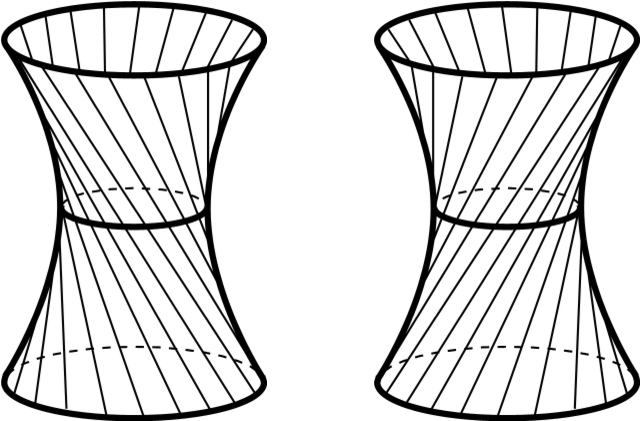
\includegraphics{./images/ch8/rtLHypo.pdf}}
		
		{\b $$\df{x^2}{a^2}+\df{y^2}{b^2}-\df{z^2}{c^2}=1$$}
 	\end{center}
\end{frame}